\documentclass[aps,prb,reprint,amsfonts,amsmath,amssymb,showpacs,groupedaddress,superscriptaddress,onecolumn]{revtex4-1}
\usepackage{bm}
\usepackage{color}
\usepackage{graphicx}
\usepackage{tabularx}
\usepackage[colorlinks,urlcolor=blue,linkcolor=blue,anchorcolor=blue,citecolor=blue,bookmarks]{hyperref}

\begin{document}

\title{Artificial two-dimensional Mott insulating superstructures with a large Mott gap: Theoretical Formalism}

\date{\today}

\maketitle

To have a better understading of the experimental observations, we construct single-band Hubbard model with renormalized hopping coefficients to describe these systems and calculate the local density of states by using cluster perturbation theory (CPT)~\cite{PhysRevB.48.418,PhysRevLett.84.522}.

For the $(3\sqrt{7} \times 3\sqrt{7})R19.1^\circ$ surface (referred to as Phase 1 in the followings), the corresponding proposed atomic structural is shown in Fig.~\ref{fig:STMTopographicImage}(g). The unit cell contains twenty-three sites while three of them are somewhat isolated, i.e., the three blue circles are speparated from the others. Considering that the hopping amplitude is inversely proportional to the square of the distance, it is reasonable to neglect the three isolated sites in a simplified model. We only include these hopping terms shown in Fig.~\ref{fig:ModelForPhase1} and the resulting Hamiltonian takes the following form:
\begin{equation}
    H = \sum_{i,j,\sigma} t_{ij}(c_{i\sigma}^{\dagger}c_{j\sigma} + \text{H.c.}) + U \sum_{i} n_{i\uparrow} n_{i\downarrow}
    \label{eq:ModelHamiltonian}
\end{equation}
where $t_{ij}$ is the effective hopping amplitude and $U$ the effective on-site Coulomb repulsion. Here, we take $t_{ij} = -1/r_{ij}^{2}$, where $r_{ij}$ is the distance between $i$-th site and $j$-site. See Appendix~\ref{appx:Coordinates} for the coordinates of these sites shown in Fig.~\ref{fig:ModelForPhase1}.

For this model Hamiltonian, we first consider the non-interacting case (\textit{i.e.,} $U = 0$) which can be diagonalized exactly. The averaged DOS and representative LDOS are shown in Fig.~\ref{fig:TBAForPhase1}. It can be clearly seen from the averaged DOS that the system has an energy gap of $\sim 0.55t$. However, the LDOS varies from site to site. For instance, the LDOS of the site labeled as ``0'' is quite different from the sites labeled as ``1'', ``2'' and ``3''. Especially, the energy gap at the zeroth site is $\sim 3.2t$, and yet that at other sites is $\sim 0.55t$. This inhomogeneous LDOS is obviously contradictory to the experimental uniform insulating gap. We further include on-site Coulomb repulsion and use CPT to calculate the LDOS. The evolution of the averaged DOS with U is shown in Fig.~\ref{fig:CPTForPhase1}. The energy gap becomes gradually decreased when taking into account of Hubbard-$U$ and a transition from band insulator to metal is identified at $U \approx 3.5t$. As we further increase $U$, an energy gap is reopened, indicating a metal-insulator transition. The including of $U = 6t$ leads to an experimentally comparable large energy gap of $\sim 2.31\text{eV}$. We further explored the corresponding LDOS and found that the energy gap is uniform at each lattice sites from 0 to 19 (see Fig.~\ref{fig:CPTForPhase1LDOS}), which is consistent with the experimentally observed homengeneous dI/dV spectra. The agreement between the experimental observation and theoretical calculation indicates the Mott origin of the large energy gap of $\sim 2.5\text{eV}$ for $(3\sqrt{7} \times 3\sqrt{7})R19.1^\circ$ surface.

For $(\sqrt{133} \times 4\sqrt{3})$ and $(13 \times 13)$ surfaces (referred to as Phase 2 and Phase 3 respectively), we similarly constructed the simplified model for theoretical calculations. Considering the substrate Si atoms form triangular lattice and the surface Sn atoms form well-ordered superstructures,we constructed Hubbard model on triangular lattice with uniformly dirtributed extra points to describe Phase 2 and Phase 3. We only consider the hopping terms between nearest-neighbor triangular lattice sites as well as the hopping terms between extra points and its' nearest neighbors. The corresponding tight-bingding model is shown in Fig.~\ref{fig:ModelForPhase2andPhase3} and the red circle correspond to the extra point. For the non-interacting part, even though the unit cell contains odd number of electrons at half-filling, the band structure and the calculated DOS indicate their metallic state with non-vanishing DOS near $E_{F}$. We further calculate the DOS of the corresponding Hubbard model by using CPT and the evolution of DOS with Hubbard-$U$ is shown in Fig.~\ref{fig:CPTForPhase2andPhase3}. With the inclusion of Hubbard-$U$, the system undergoes an metal-insulator transition at $U \approx 2t$. When we further increase $U$ to $6t$ to be consistent with the value of Phase 1, the Mott gap is about $3.84t$. The calculated gap size of
Phase 2 and Phase3 is larger than the gap size of Phase 1, which is qualitatively consistent the experimental onservation. Due to the fact that the actual atomic arrangements are slightly deviated from the proposed model, we introduce randomness on the hopping amplitude to study the influence of deviations of the atomic positions, i.e., we set the hopping coefficients $t_{ij} = -A / r_{ij}$ where $r_{ij}$ is the distance between the $i$-th and $j$-th lattice sites and $A$ is random number. We can set the hopping amplitude to be in different range and the corresponding DOS are shown in Fig.~\ref{fig:CPTForPhase2andPhase3Random}. It can be seen from Fig.~\ref{fig:CPTForPhase2andPhase3Random}, random sampling of hopping amplitude $A$ only has sightly influence on the resulting DOS which implies that the tiny influence of the deviation of the atomic positions. In addition, the theoretical calculations of the LDOS with $U = 6t$ at different lattice sites show the constant Mott gap, same as the uniform dI/dV spectra obseraved experimentally. The good agreements furhter confirm these two superstructures are also large-gap Mott insulators.


\begin{figure}[p]
    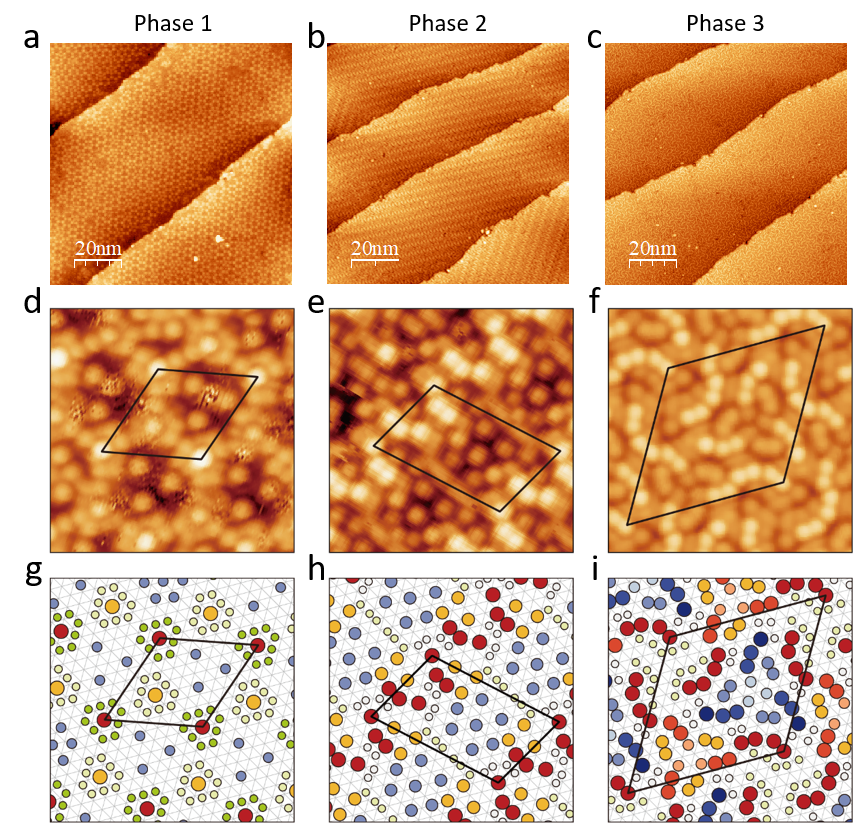
\includegraphics[width=0.8\columnwidth]{STMTopographicImage.png}
    \caption{\label{fig:STMTopographicImage}(Color online) STM characterization of three new superstructures of Sn sub-monolayers on Si(111). (a)-(c) Large-scale STM image (size: 100 $\times$ 100 nm$^2$) taken on $(3\sqrt{7} \times 3\sqrt{7})R19.1^\circ$, $(\sqrt{133} \times 4\sqrt{3})$ and $(13 \times 13)$ surfaces. They are taken at $U = +3.5V$, $U = -2V$ and $U = -2V$ ($I_{t} = 100pA$) respectively. (d)-(f) The atomically resolved STM images of them taken at $U = -2V, I_{t} = 200pA$. The surface unit cells of them are marked in black. (g)-(i) The corresponding proposed atomic structural models. The marked surface unit cells in (g)-(i) are the same as these in (d)-(f).}
\end{figure}

\begin{figure}[p]
    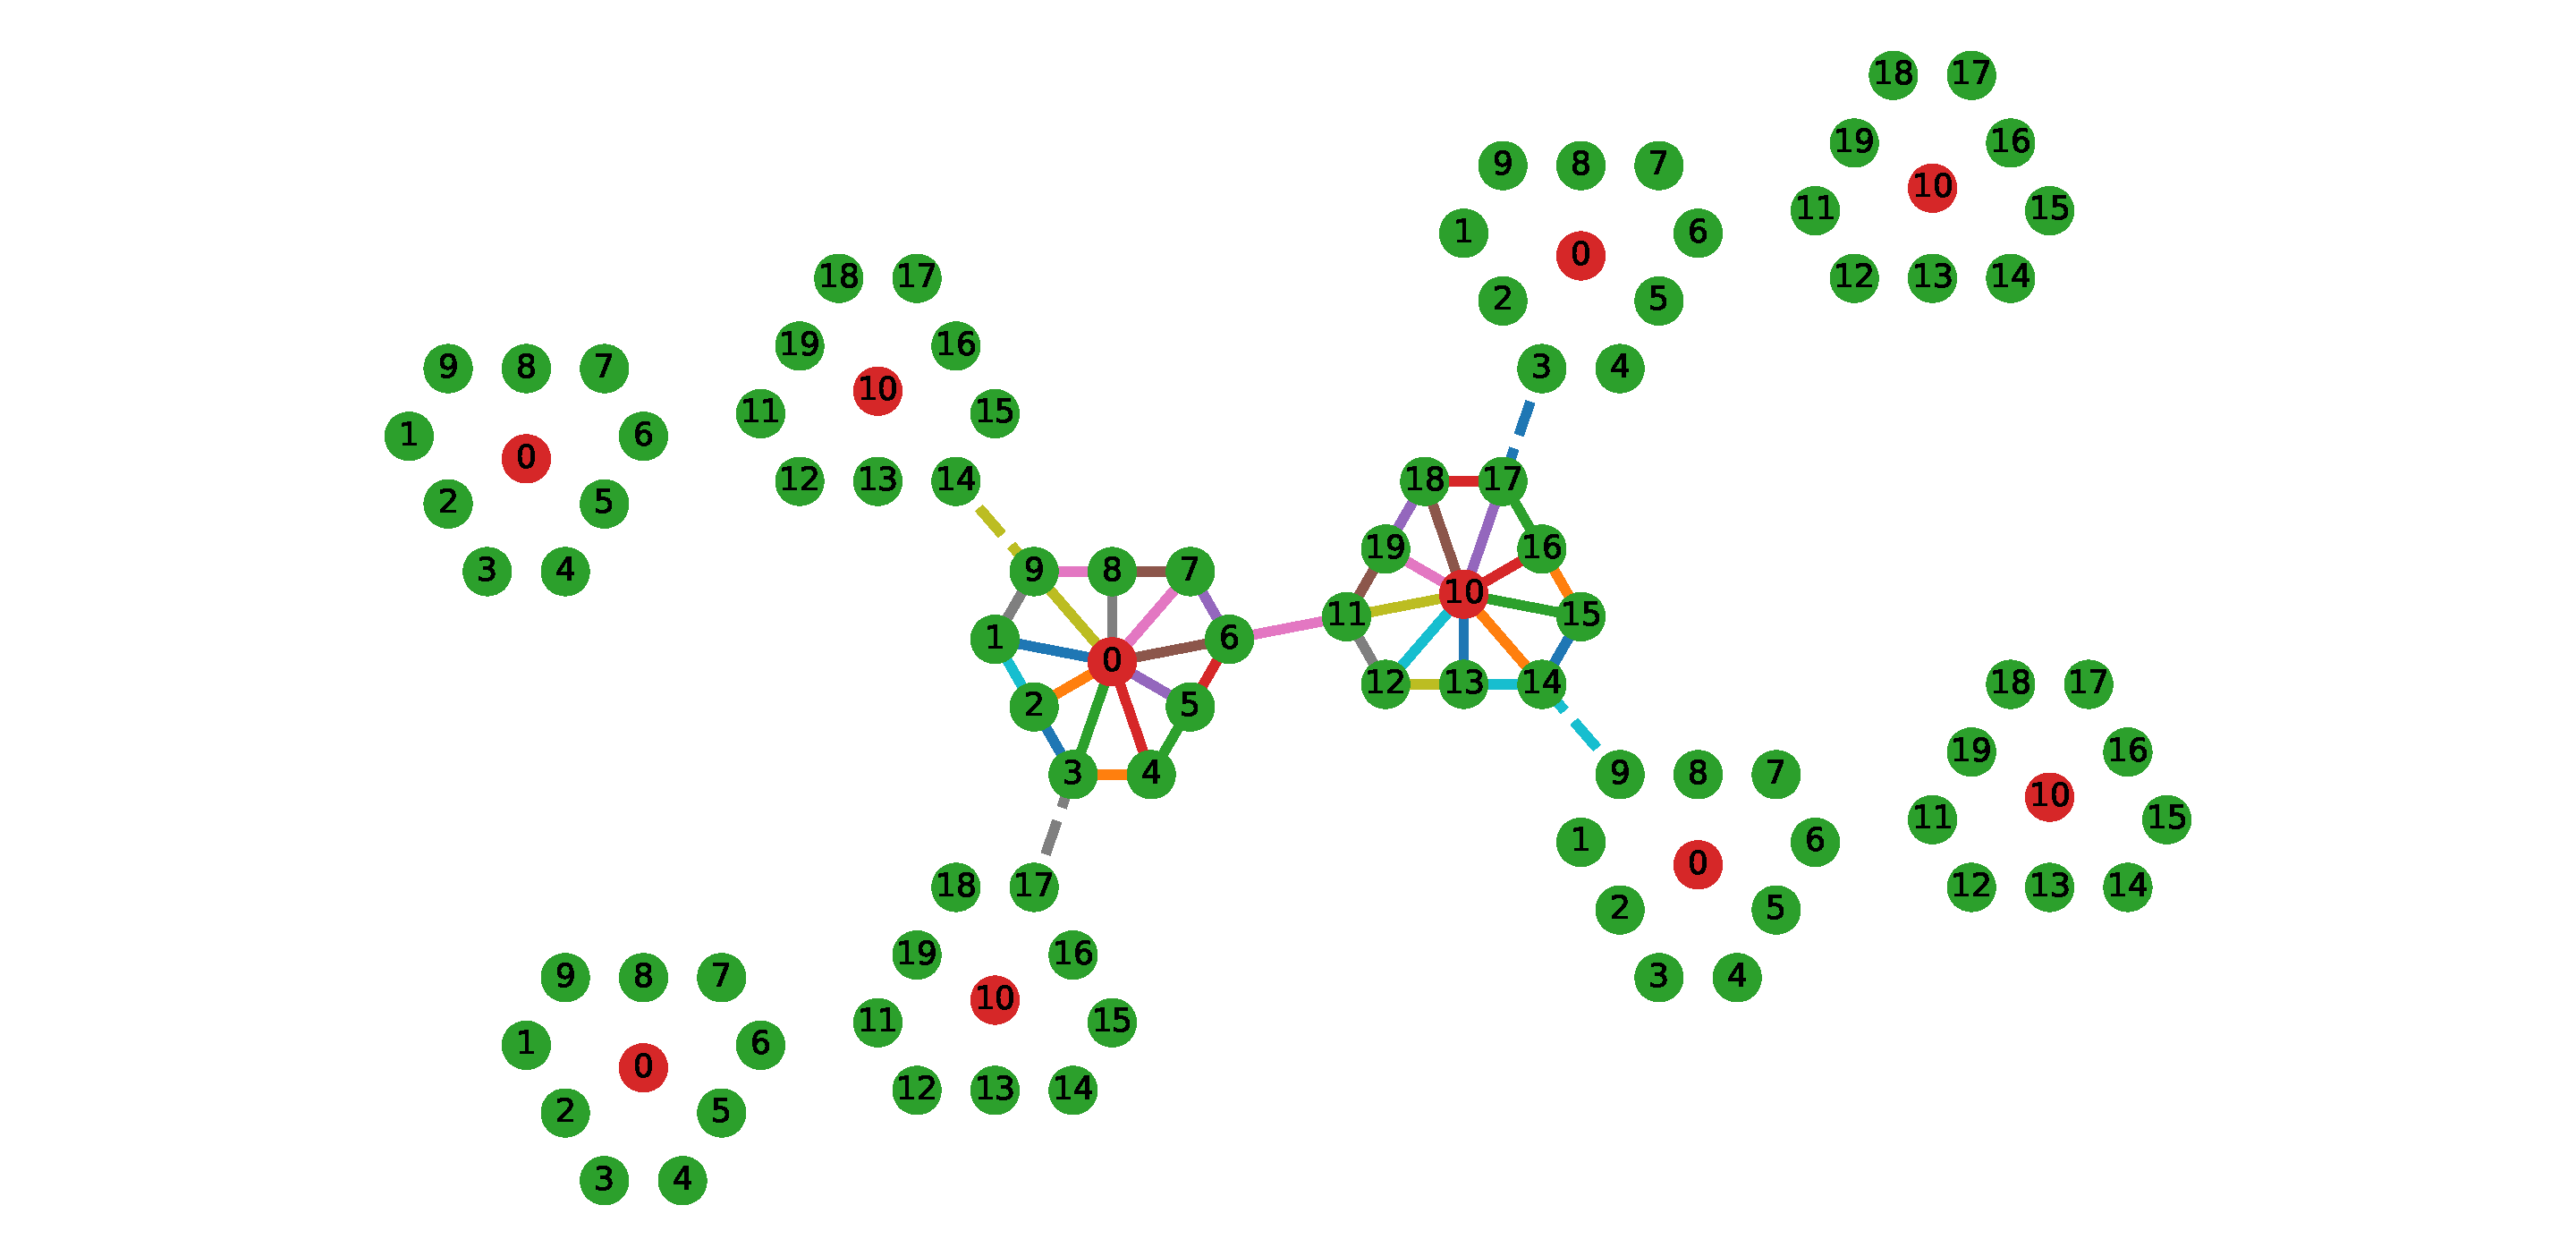
\includegraphics[width=0.8\columnwidth]{ModelForPhase1.pdf}
    \caption{\label{fig:ModelForPhase1} (Color online) Demonstration of the hopping terms for Phase 1. The unit cell has twenty sites labeled from 0 to 19. The soild and dashed lines correspond to the hopping terms $t_{ij} (c_{i\sigma}^{\dagger} c_{j\sigma} + \text{H.c.})$, where $t_{ij} = -1/r_{ij}^{2}$ and $r_{ij}$ is the distance from $i$-th to $j$-th site.}
\end{figure}

\begin{figure}[p]
    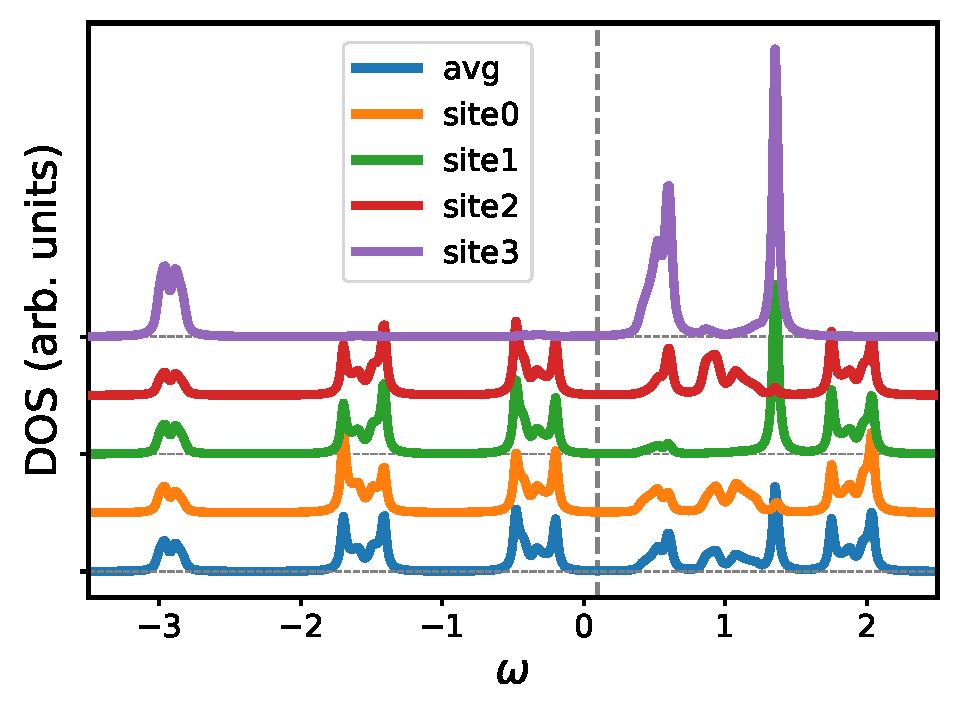
\includegraphics[width=0.8\columnwidth]{TBAForPhase1.pdf}
    \caption{\label{fig:TBAForPhase1} (Color online) Local density of states calculated from the tight-binding model defined in Fig.~\ref{fig:ModelForPhase1}. The blue line is the average of the LDOS over the twenty sites in a unit cell. LDOS for site \{0, 10\}, \{1, 4, 7, 12, 15, 18\}, \{2, 5, 8, 13, 16, 19\}, \{3, 6, 9, 11, 14, 17\} are the same. The gray dashed vertical line marks the Fermi energy $E_{F}$.}
\end{figure}

\begin{figure}[p]
    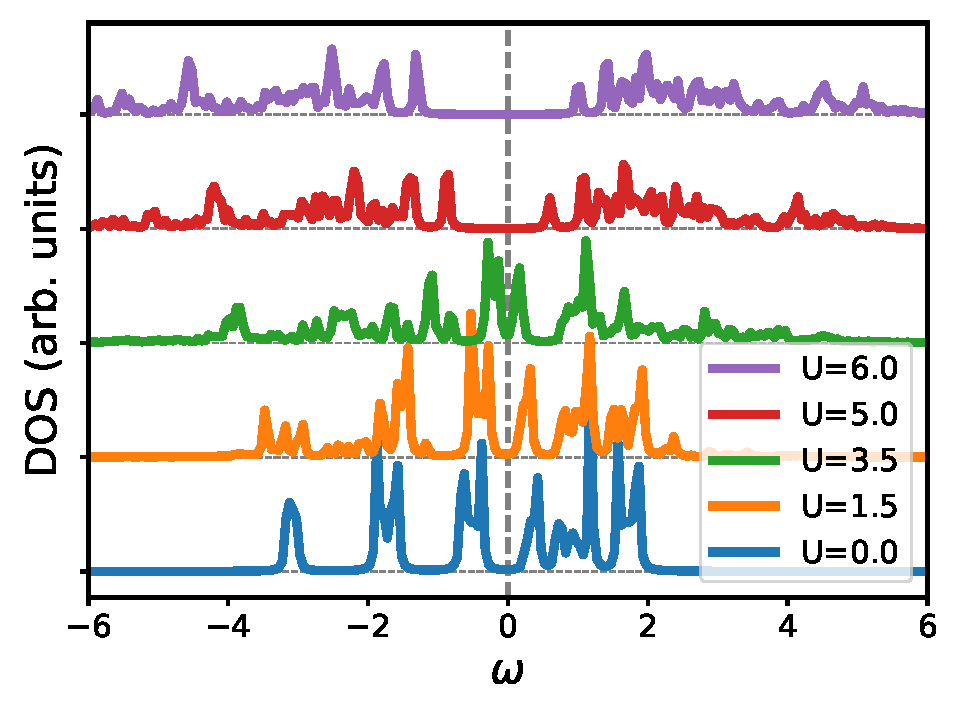
\includegraphics[width=0.8\columnwidth]{CPTForPhase1.pdf}
    \caption{\label{fig:CPTForPhase1} (Color online) The evolution of averaged DOS with Hubbard-$U$.}
\end{figure}

\begin{figure}[p]
    \centering
    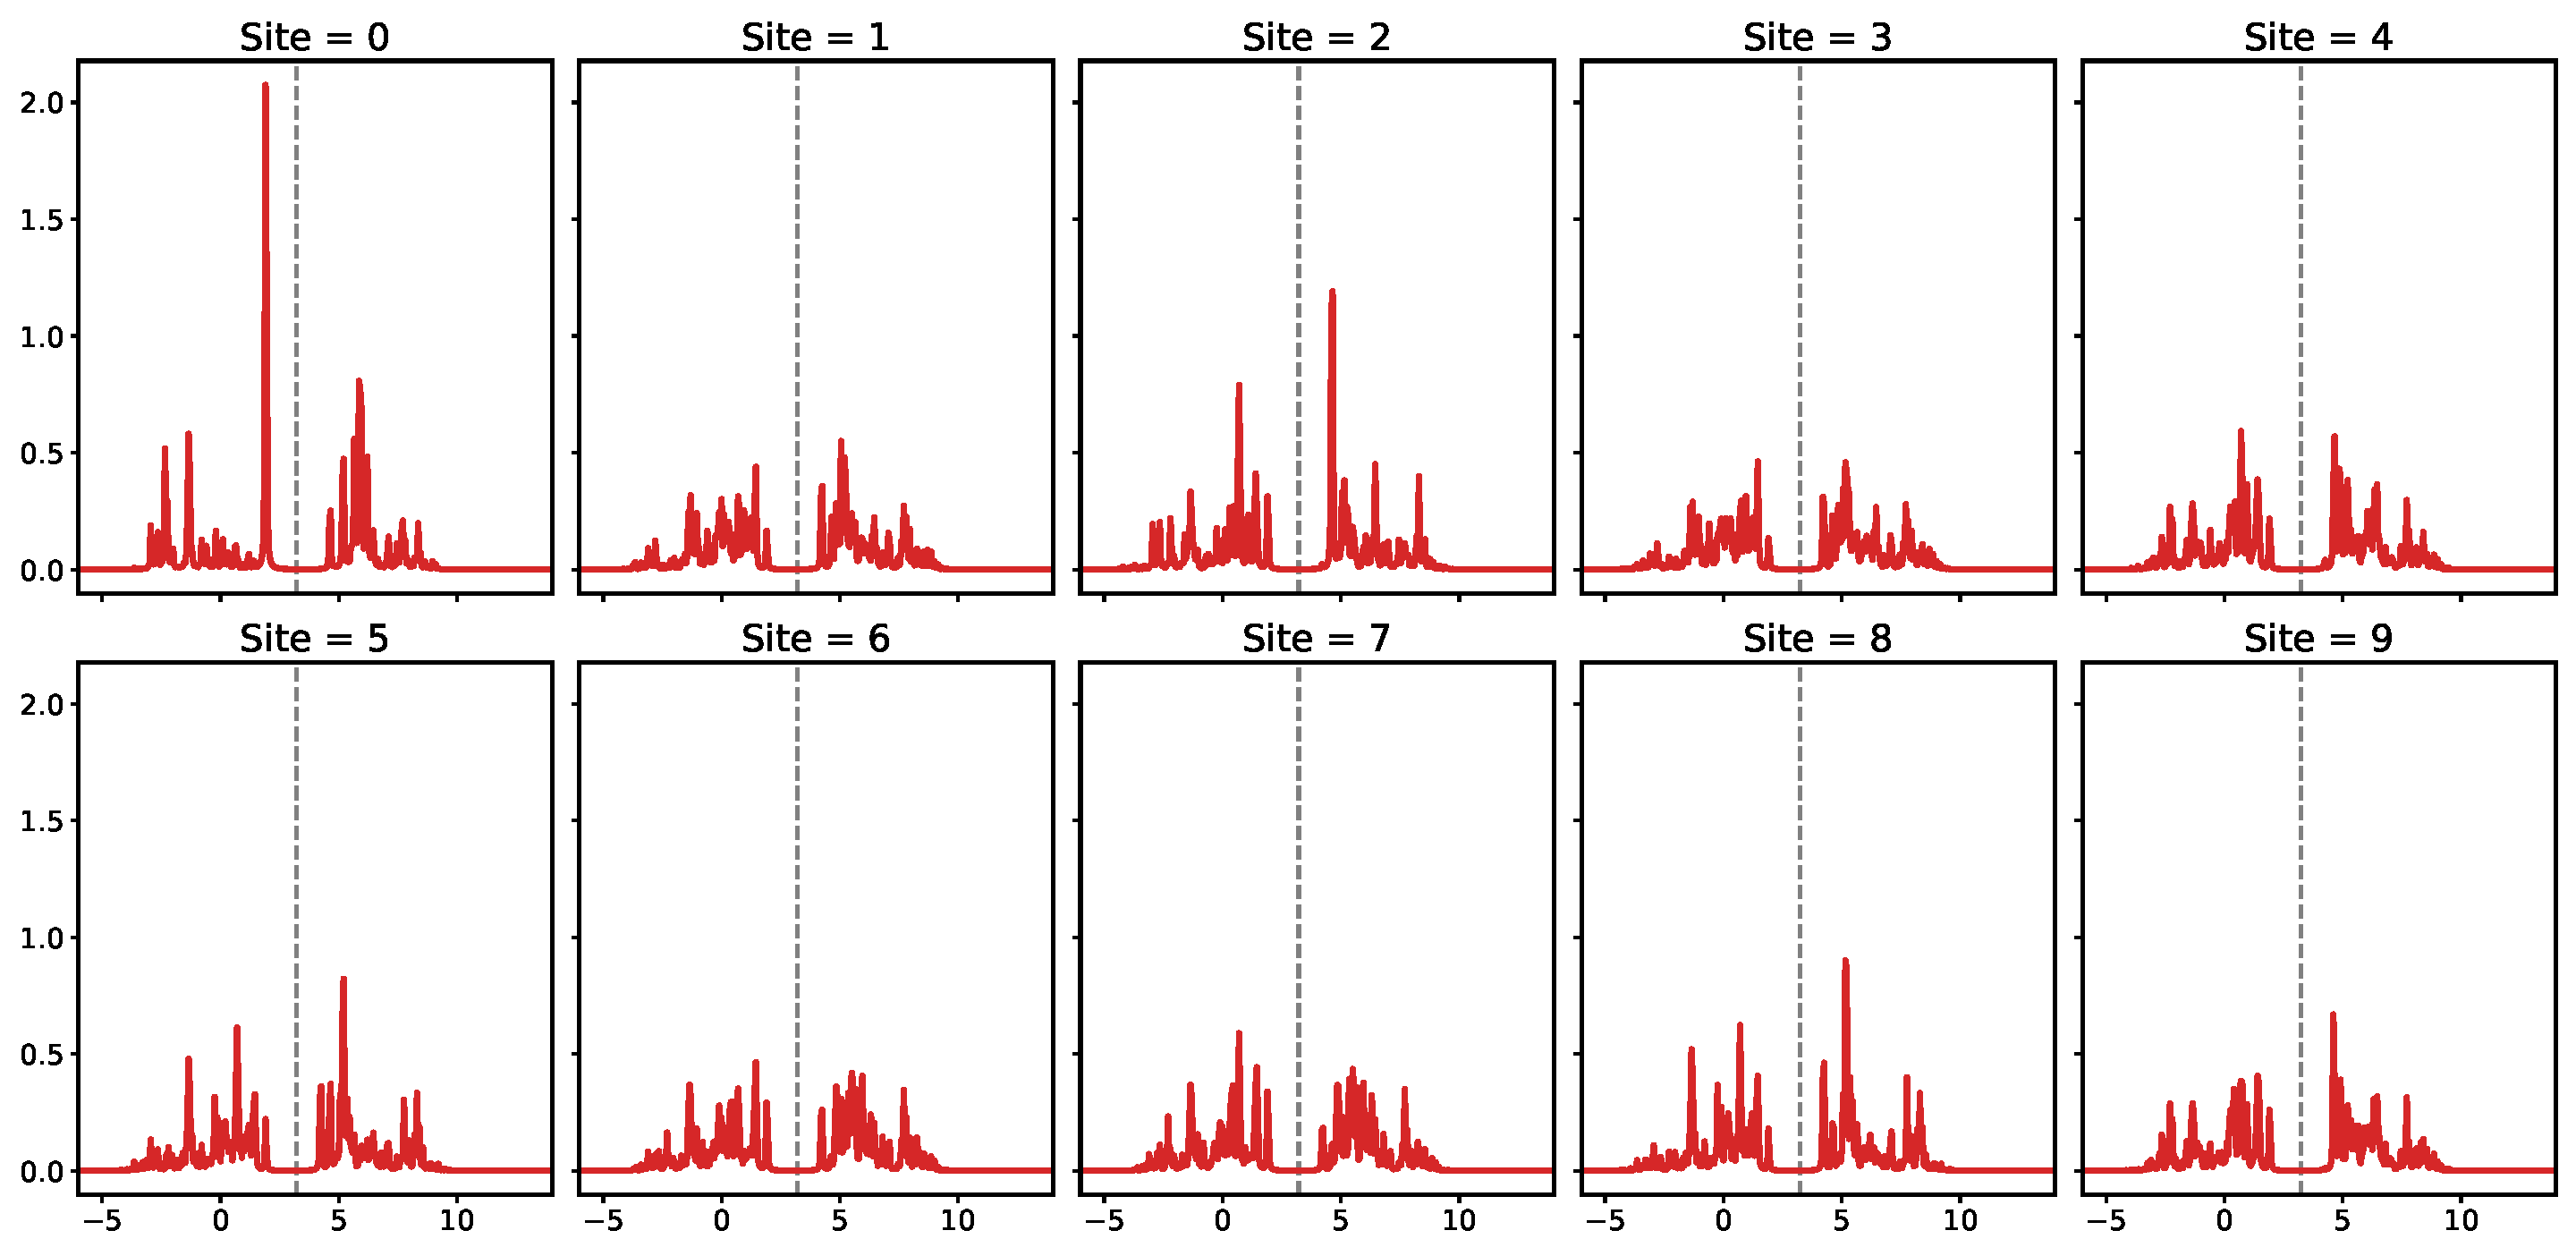
\includegraphics[width=0.8\columnwidth]{CPTForPhase1LDOS0.pdf}
    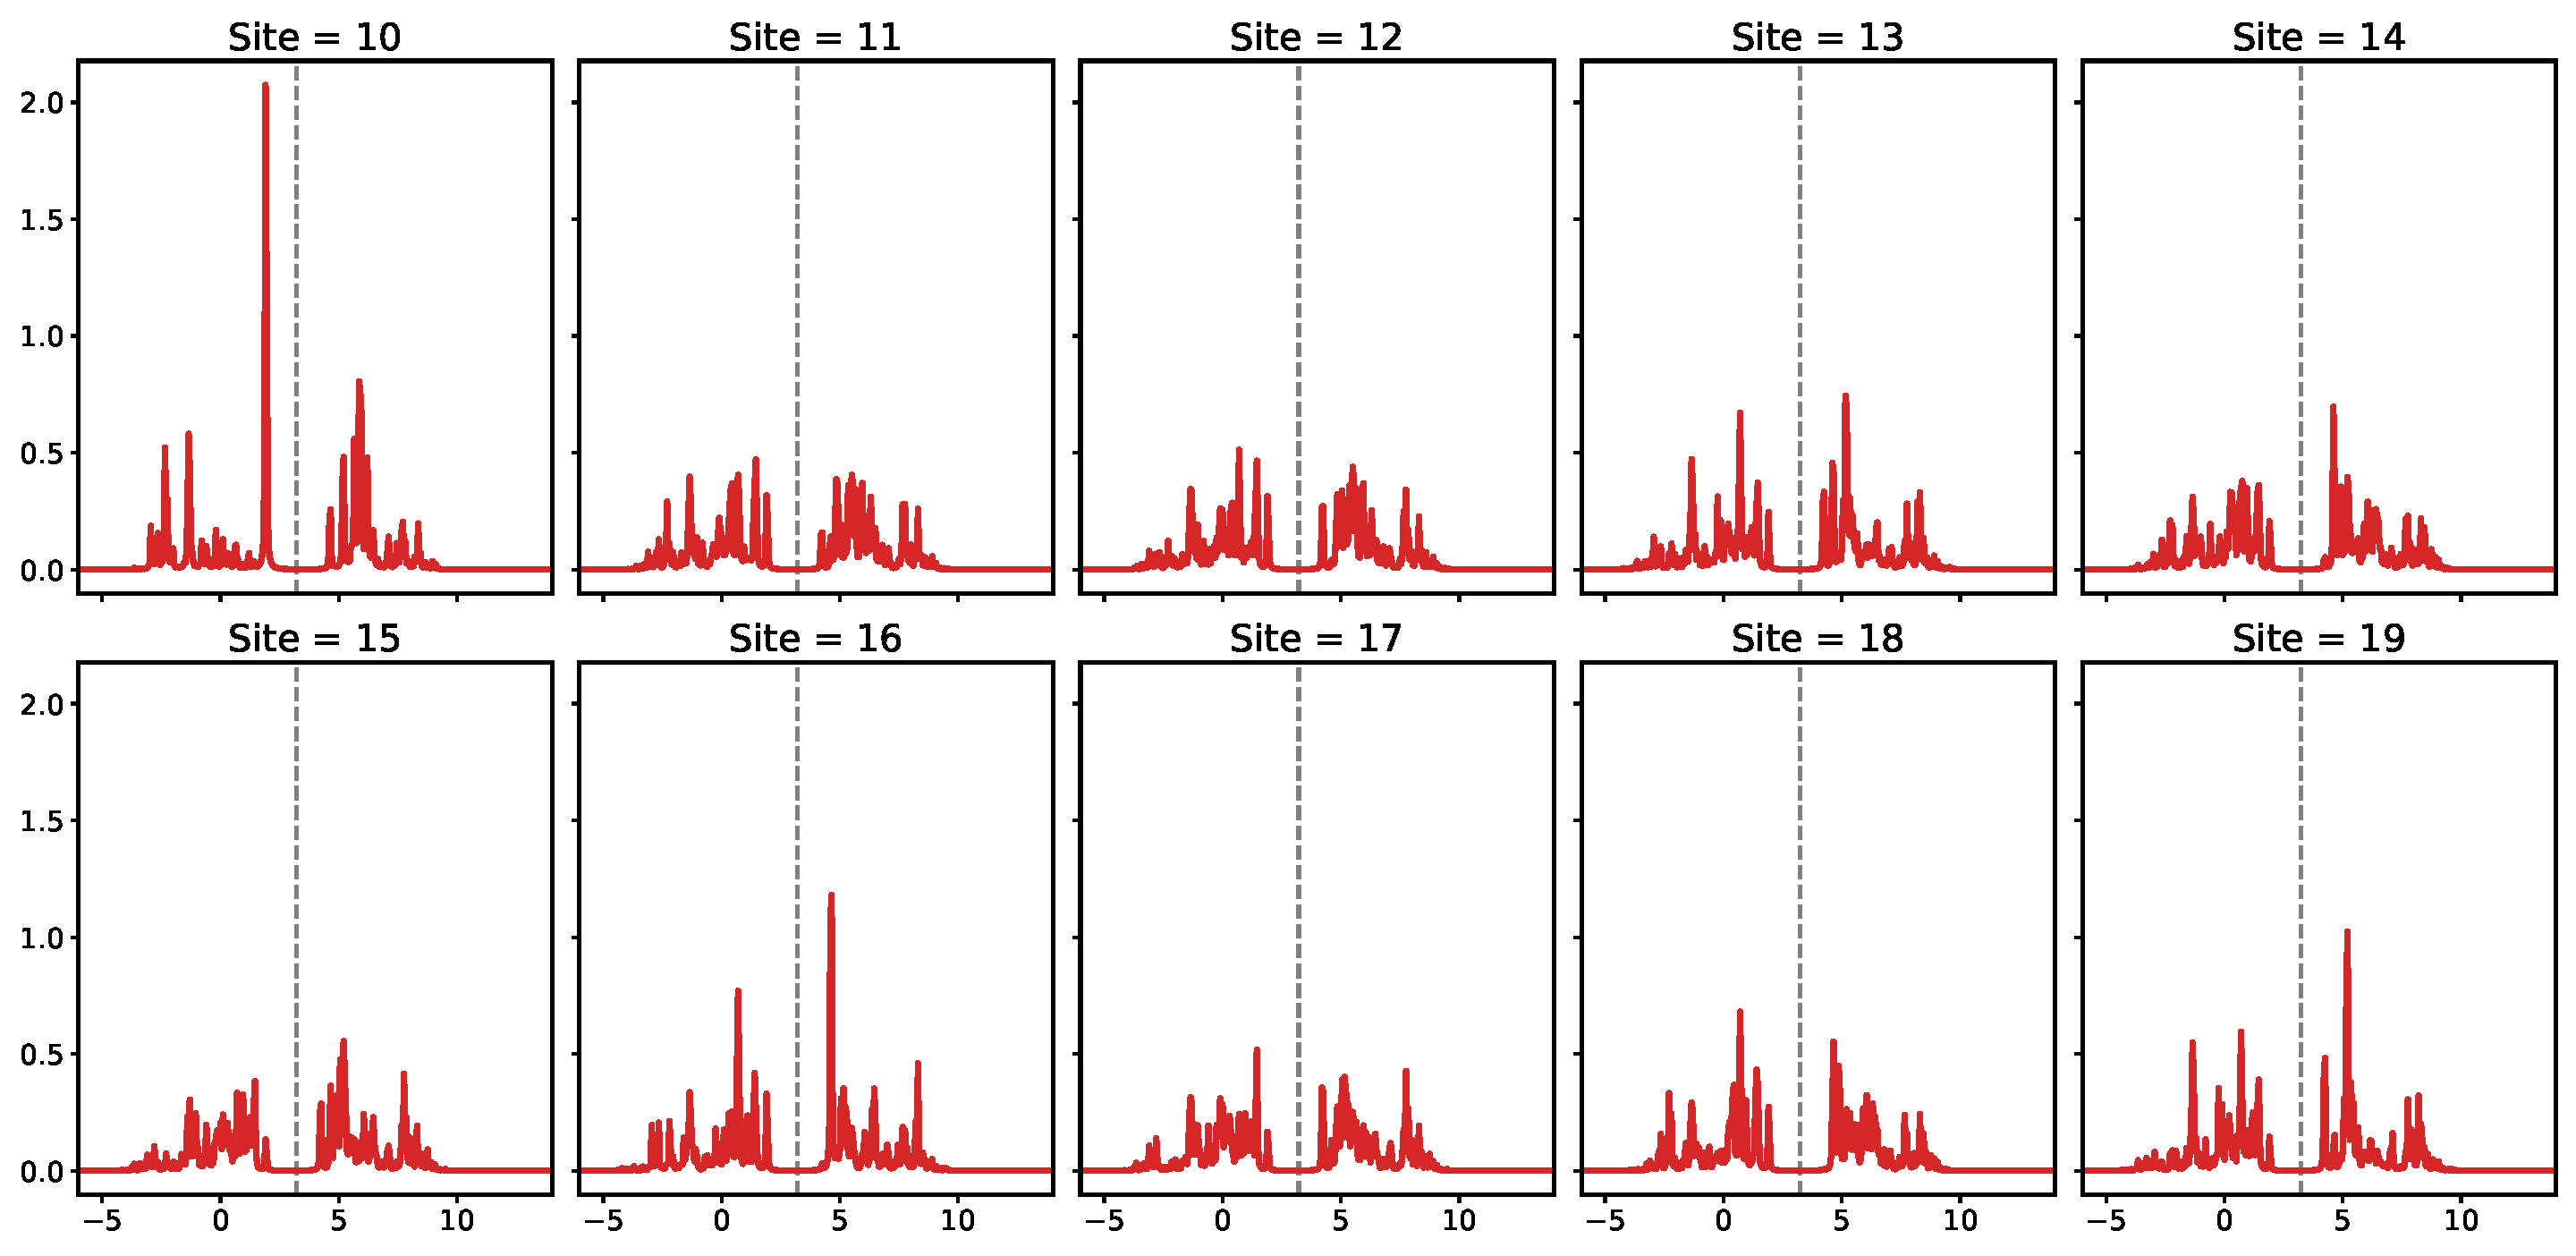
\includegraphics[width=0.8\columnwidth]{CPTForPhase1LDOS1.pdf}
    \caption{\label{fig:CPTForPhase1LDOS} Local density of states at $U = 6t$.}
\end{figure}

\begin{figure}[p]
    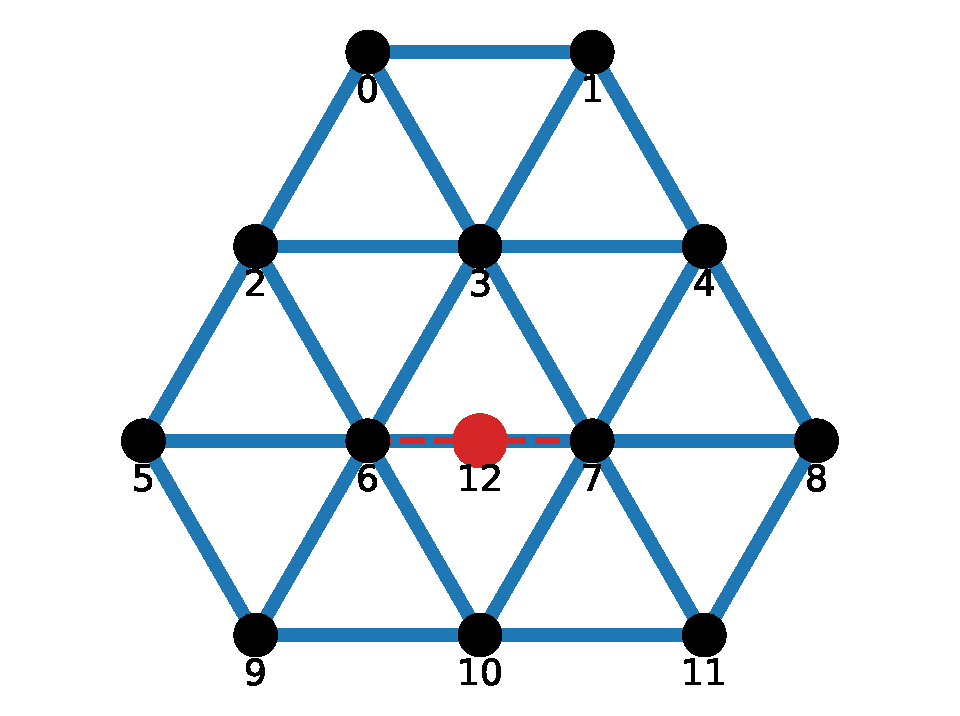
\includegraphics[width=0.8\columnwidth]{ModelForPhase2andPhase3.pdf}
    \caption{\label{fig:ModelForPhase2andPhase3} (Color online) Demonstration of the tight-binding model for Phase 2 and Phase 3. The soild and dashed lines correspond to the hopping terms $t_{ij} (c_{i\sigma}^{\dagger} c_{j\sigma} + \text{H.c.})$, where $t_{ij} = -1/r_{ij}^{2}$ and $r_{ij}$ is the distance from $i$-th to $j$-th site.}
\end{figure}

\begin{figure}[p]
    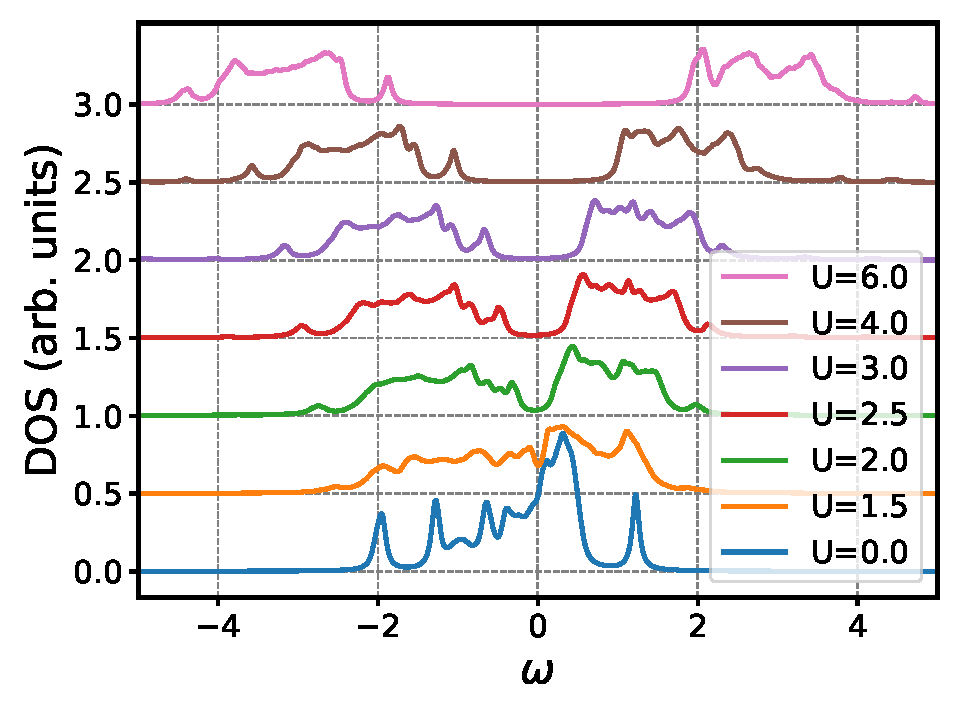
\includegraphics[width=0.8\columnwidth]{CPTForPhase2andPhase3.pdf}
    \caption{\label{fig:CPTForPhase2andPhase3} (Color online) The evolution of averaged DOS with Hubbard-$U$.}
\end{figure}

\begin{figure}
    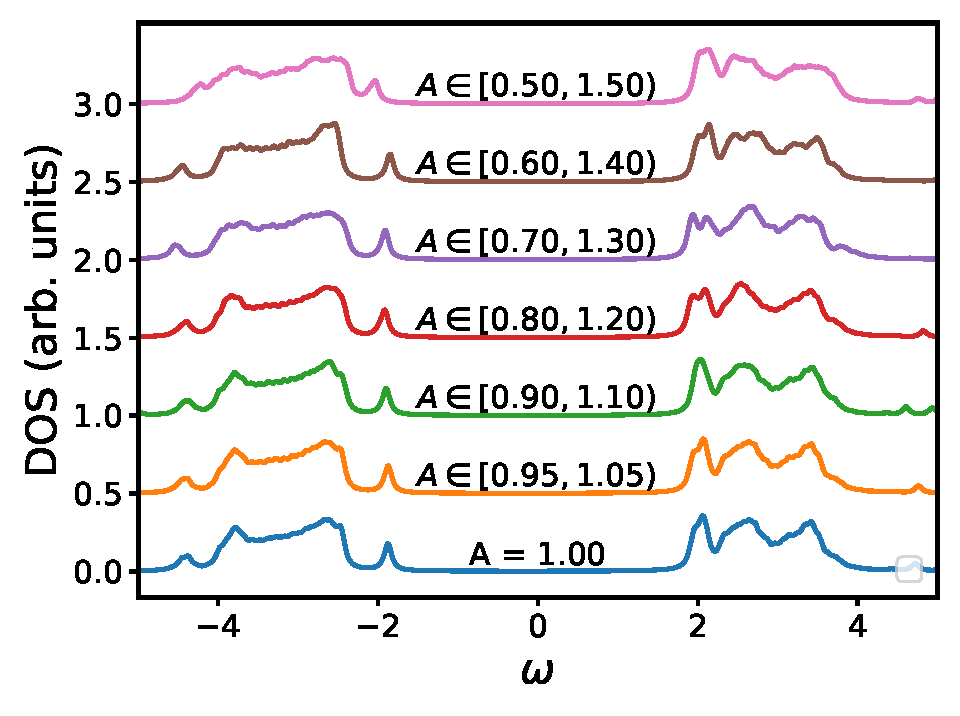
\includegraphics[width=0.8\columnwidth]{CPTForPhase2andPhase3Random.pdf}
    \caption{\label{fig:CPTForPhase2andPhase3Random} (Color Online) DOS at $U = 6t$ with random hopping amplitude.}
\end{figure}

\appendix

\section{\label{appx:Coordinates}Coordinates of these sites in Phase 1}

\begin{table}[h]
    \centering
    \begin{tabular}{c | l | c | l}
        \hline
        index & (x, y) & index & (x, y) \\
        \hline
        0 & (0, 0) & 1 & (-1.5, $\sqrt{3} / 6$) \\
        \hline
        2 & (-1.0, -$\sqrt{3}$ / 3) & 3 & (-0.5, -5$\sqrt{3}$ / 6) \\
        \hline
        4 & (0.5, -5$\sqrt{3}$ / 6) & 5 & (1.0, -$\sqrt{3}$ / 3) \\
        \hline
        6 & (1.5, $\sqrt{3}$ / 6) & 7 & (1.0, 2$\sqrt{3}$ / 3) \\
        \hline
        8 & (0.0, 2$\sqrt{3}$ / 3) & 9 & -1.0, 2$\sqrt{3}$ / 3 \\
        \hline
        10 & (4.5, $\sqrt{3}$ / 2) & 11 & (3.0, $\sqrt{3}$ / 3) \\
        \hline
        12 & (3.5, -$\sqrt{3}$ / 6) & 13 & (4.5, -$\sqrt{3}$ / 6) \\
        \hline
        14 & (5.5, -$\sqrt{3}$ / 6) & 15 & (6.0, $\sqrt{3}$ / 3) \\
        \hline
        16 & (5.5, 5$\sqrt{3}$ / 6) & 17 & (5.0, 4$\sqrt{3}$ / 3) \\
        \hline
        18 & (4.0, 4$\sqrt{3}$ / 3) & 19 & (3.5, 5$\sqrt{3}$ / 6) \\
        \hline
        20 & (8.0, $\sqrt{3}$ / 3) & 21 & (10.5, 5$\sqrt{3}$ / 6) \\
        \hline
        22 & (8.5, 11$\sqrt{3}$ / 6) & & \\
        \hline
    \end{tabular}
    \caption{\label{tab:Coordinates}Coordinates of these sites in Phase 1.}
\end{table}


\bibliography{TheoreticalFormalism}

\end{document}
